\documentclass[11pt,a4paper]{article}
\usepackage{cite}
\usepackage{color}
\usepackage{graphicx}
\usepackage{amsmath}
\usepackage[margin=1in]{geometry}

\title{The BRG Visual-Inertial Odometry Documentation}
\author{David Hanley, Alex Faustino, David Degenhardt, Tim Bretl}

\begin{document}
\maketitle

\begin{abstract}
 The purpose of this article is to document the approach to the Bretl Research Group's visual-inertial odometry method. To develop this method we test using a segment of the Euroc dataset.
\end{abstract}

\section{Introduction}

\subsection{Coordinate Systems}

\subsection{A Note on Quaternion Conventions}
Note that our VIO method uses the JPL convention for quaternions as opposed to Hamilton's convention. For more details regarding this convention, see \cite{Trawny:2005,Barfoot:2011,Wie:2008}. Our performance evaluation code requests the user to input the quaternion convention used for state estimation and for the ground truth. So, comparisons with of our VIO result with Hamilton-convention ground truth can be easily done. 

\subsection{Peformance Evaluation}
We evaluate performance using measure of the relative pose error (RPE) of the translational state estimate over 100 time intervals. Each interval will have at least 20 measurments of RPE. We then plot RPE as a function of the time interval at 25\%, 50\%, and 75\% quartiles. This RPE is computed as defined by  \cite{Sturm:2012}. Given a time interval $\Delta$, ground truth pose $Q\in SE(3)$, and estimated pose $P\in SE(3)$, at time step $i$ the RPE is computed as
\begin{equation}
	E_i = \left(Q_i^{-1}Q_{i+\Delta}\right)^{-1}\left(P_i^{-1}P_{i+\Delta}\right).
\end{equation}
This code is currently in the $\texttt{perf\_eval}$ folder and is written in Matlab. When running the $\texttt{rpe\_main.m}$ script, one simply has to type the name of the ground truth and estimated pose files. The files must be moved into the $\texttt{perf\_eval}$ directory. Figure \ref{fig:exampleresult} show an example of the output of the performance evaluation script.

\begin{figure}
	\centering
	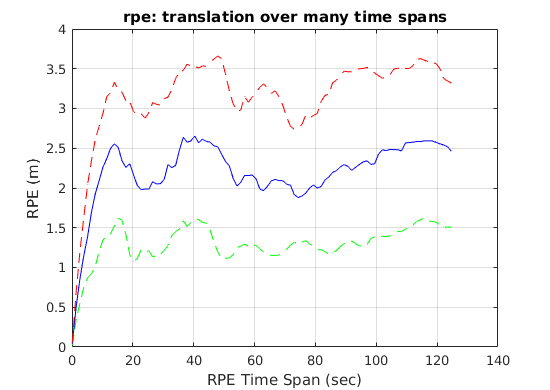
\includegraphics[scale=0.6]{example_result}
	\caption{We evaluate our result by computing translational RPE (i.e. $\|trans(E_i)\|$) for a set of time spans ($\Delta$). The dashed red line shows the 75 percent quartile, the solid blue line is the median, and the dashed blue line is the 25 percent quartile.}
	\label{fig:exampleresult}
\end{figure}

\section{Conclusion}

blah blah blah 

\bibliographystyle{IEEEtran}
\bibliography{IEEEabrv,references}

\end{document}